\documentclass[a4paper, 12pt]{article}

\usepackage[utf8]{inputenc}
\usepackage[T1, T2A]{fontenc}
\usepackage[english, russian]{babel}
\usepackage[top=2cm, bottom=2cm, left=2cm, right=2cm]{geometry}

\usepackage{pgfplots}
\usepgfplotslibrary{polar}
\pgfplotsset{compat=1.13}
\pgfplotsset{grid = major, grid style = {dashed}}
\usepackage{pscyr}
\usepackage{subcaption}
\usepackage{amsmath}

\usepackage{tabu}

\usepackage{float}

% PGFPlots Table ========================================================
\usepackage{pgfplotstable}
\renewcommand{\arraystretch}{1.3}
% recommended:
\usepackage{booktabs}
\usepackage{colortbl}
% pgfplotstable settings
\pgfplotstableset{
    every head row/.style = {before row = \hline},
    after row = {[1mm] \hline},
    column type = {|c},
    every last column/.style={
        column type/.add={}{|},
    },   
}
\usepackage{threeparttable}
\renewcommand{\TPTminimum}{0.6\linewidth}

% Paragraph indent
\usepackage{indentfirst}
\setlength{\parindent}{15mm}

%Change label separator
\usepackage{caption}
\captionsetup[table]{labelformat=simple, labelsep = endash, justification = raggedright, singlelinecheck = off, width = 0.75\textwidth}
\captionsetup[figure]{labelformat=simple, labelsep = endash, name = Рисунок}
\newcommand\tline[2]{$\underset{\text{#1}}{\text{\underline{\hspace{#2}}}}$}

\begin{document}
	\begin{titlepage}
		\centering
		{\fontsize{12pt}{5cm}\selectfont \bfseries Министерство образования и науки Российской Федерации} \\ \vspace{0.5cm}
		{\fontsize{7pt}{5cm}\selectfont ФЕДЕРАЛЬНОЕ ГОСУДАРСТВЕННОЕ АВТОНОМНОЕ ОБРАЗОВАТЕЛЬНОЕ УЧРЕЖДЕНИЕ ВЫСШЕГО ПРОФЕССИОНАЛЬНОГО ОБРАЗОВАНИЯ} \\ 
		\vspace{1cm}
		{\fontsize{12pt}{5cm}\selectfont \bfseries САНКТ-ПЕТЕРБУРГСКИЙ УНИВЕРСИТЕТ ИНФОРМАЦИОННЫХ ТЕХНОЛОГИЙ, МЕХАНИКИ И ОПТИКИ} \\ \vspace{1.5cm}

		{\fontsize{14pt}{5cm}\selectfont Кафедра \hspace{1cm} \underline{Систем Управления и Информатики}  \hspace{1cm} Группа \underline{Р3340}} \\ 
		\vspace{2cm}

		{\fontsize{20pt}{5cm}\selectfont \bfseries Лабораторная работа №12} \\
		{\fontsize{20pt}{5cm}\selectfont \bfseries “Анализ линейных непрерывных систем с использованием прикладного пакета Matlab Control System Toolbox”} \\
		{\fontsize{14pt}{5cm}\selectfont Вариант - 7} \\
		\vspace{1.5cm}

		\flushleft

		{Выполнил \hspace{2cm} \tline{(фамилия, и.о.)}{9cm} (подпись)} \\
		\vspace{2cm}

		{Проверил \hspace{2cm} \tline{(фамилия, и.о.)}{9cm} (подпись)} \\
		\vspace{5cm}

		"\underline{\hspace{0.7cm}}"\hspace{0.2cm}\underline{\hspace{2cm}}\hspace{0.2cm}20\underline{\hspace{0.7cm}}г. \hspace{2cm} Санкт-Петербург, \hspace{2cm} 20\underline{\hspace{0.7cm}}г. \\ \vspace{1cm}

		Работа выполнена с оценкой \hspace{1cm} \underline{\hspace{8cm}} \\ 
		\vspace{1cm}
		Дата защиты "\underline{\hspace{0.7cm}}"\hspace{0.2cm}\underline{\hspace{2cm}}\hspace{0.2cm}20\underline{\hspace{0.7cm}}г.

\end{titlepage}

\begin{center}
\section*{Задача}
\end{center} \par
\textbf{Целью работы} является исследование динамических и частотных характеристик, анализ структурных свойств и устойчивости линейных непрерывных систем с помощью прикладного пакета matlab. \par
В качестве объекта исследования выбраны линейные непрерывные динамические стационарные системы. Исходная модель разомкнутой системы представляется в форме вход-выход и описывается передаточной функцией вида: 
\begin{equation} 
    W(s) = \frac{b_1s + b_0}{s(a_2s^2 + a_1s + a_0)}
\end{equation} \par
Значения коэффициентов $a_0, a_1, a_2, b_0, b_1$ представлены в таблице 1. \par
\begin{table} [h!]
    \centering
    \begin{threeparttable}
        \caption{Коэффициенты передаточной функции}
        \begin{tabular}{|c|c|c|c|c|}
            \hline
            $a_0$ & $a_1$ & $a_2$ & $b_0$ & $b_1$ \\ \hline
            4 & 3 & 2 & 1 & 2 \\ \hline
        \end{tabular}
    \end{threeparttable}
\end{table}

\newpage
\begin{center}
\section{Анализ разомкнутой системы}
\end{center} \par
Передаточная функция разомкнутой системы представлена ниже:
\begin{equation}
    W(s) = \frac{2s + 1}{2s^3 + 3s^2 + 4s}
\end{equation}

\par 
Из исходной системы можем найти нули и полюса.
    \begin{align*}
        p_1 & = -0.5 \\
        z_1 & = 0 & z_{2, 3} = -0.7321 \pm j1.249
    \end{align*}
    где p - полюса, z - нули. Графическое изображение найденых решений представлено на рисунке 1.
    
    \begin{figure} [h!]
        \centering
		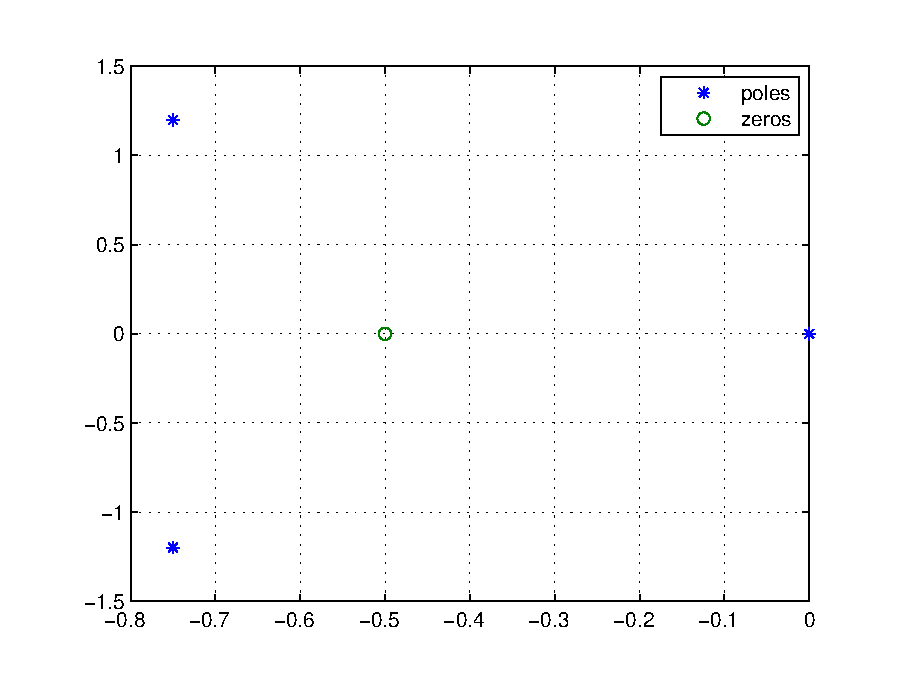
\includegraphics[scale=0.9]{image/pole1.eps}
        \caption{Нули и полюса}
    \end{figure}

\par 
Далее построим логарифмические амплитудночастотные и фазочастотные характеристики. Они представлены на рисунке 2.

\newpage
\begin{figure}[h!]
    \centering
    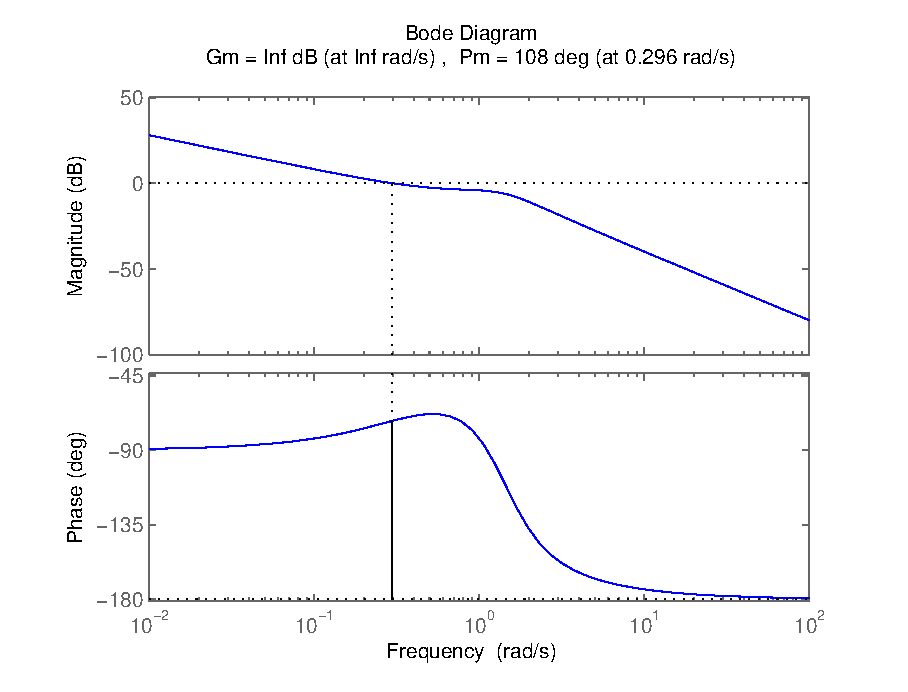
\includegraphics[scale=1.0]{image/bode.eps}
	\caption{ЛАЧХ и ЛФЧХ}
\end{figure}
\par 
График АФЧХ представлен на рисунке 3. По графику видно, что АФЧХ не охватывает точку $(-1; j0)$, а значит, является устойчивой по критерию Найквиста.
    \begin{figure}[h!]
    \centering
	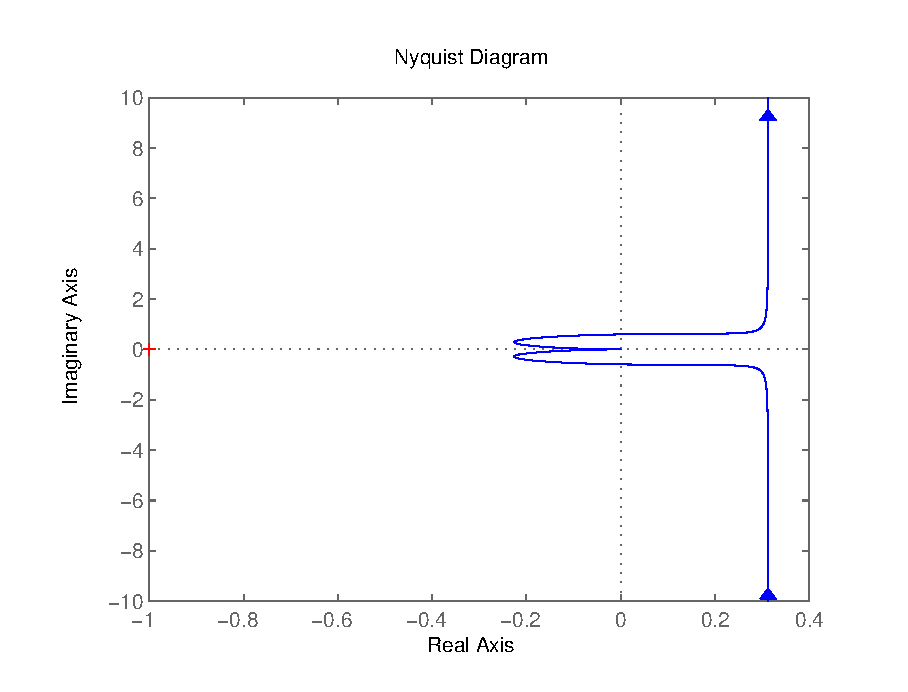
\includegraphics[scale=0.9]{image/nyquist.eps}
    \caption{АФЧХ}
    \end{figure}

\newpage
\begin{center}
\section{Анализ замкнутой системы}
\end{center} \par

Передаточная функция с коэффициентом обратной связи $K$ записана ниже.
\begin{equation}
    W_\text{замк.}(s) = \frac{2s + 1}{2s^3 + 3s^2 + (4+2K)s + K}
\end{equation} \par
Далее на рисунке 4 представлен графики корней и полюсов при разных коэффициентах обратой связи. \par
\begin{figure} [h!]
    \centering
	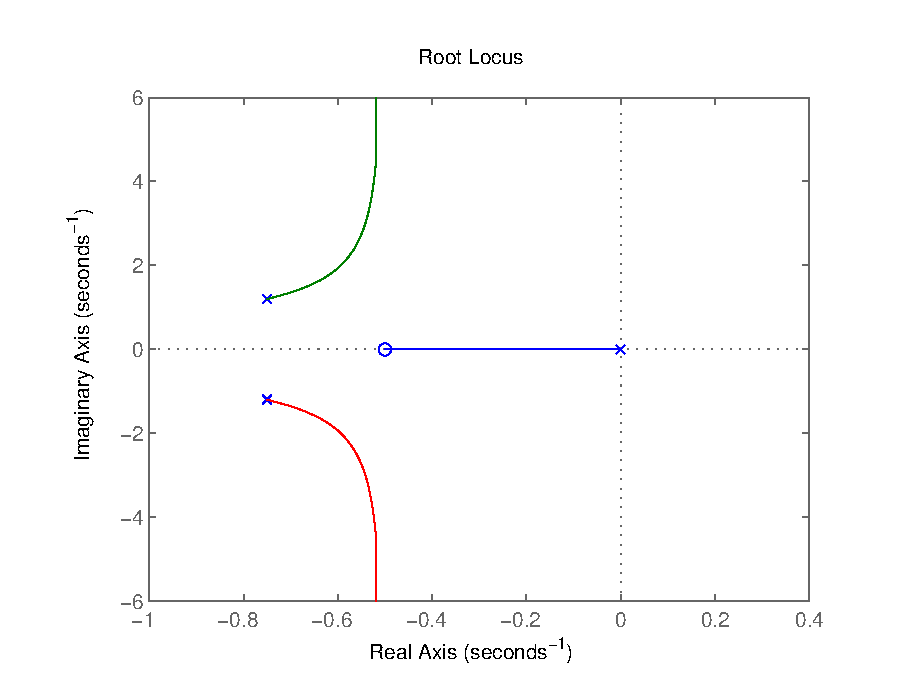
\includegraphics[scale=0.9]{image/rlocust.eps}
    \caption{Нули и полюса}
\end{figure}
\par 
Для нахождения коэффициента $K$, при котором система будет устойчивой, составим матрицу Гурвица:
\begin{equation}
	\text{Г}= \left|
	\begin{array}{ccc}
		3 & K & 0\\
		2 & 4+2K & 0\\
		0 & 3 & K\\
	\end{array}
	\right|.
\end{equation}
\par 
По критерию Гурвица получаем, что система будет асимптотически устойчива при $K > 0$ и находиться на нейтральной границе устойчивости при $K=0$. Выберем $K=2.5$.
    \begin{figure} [H]
        \centering
		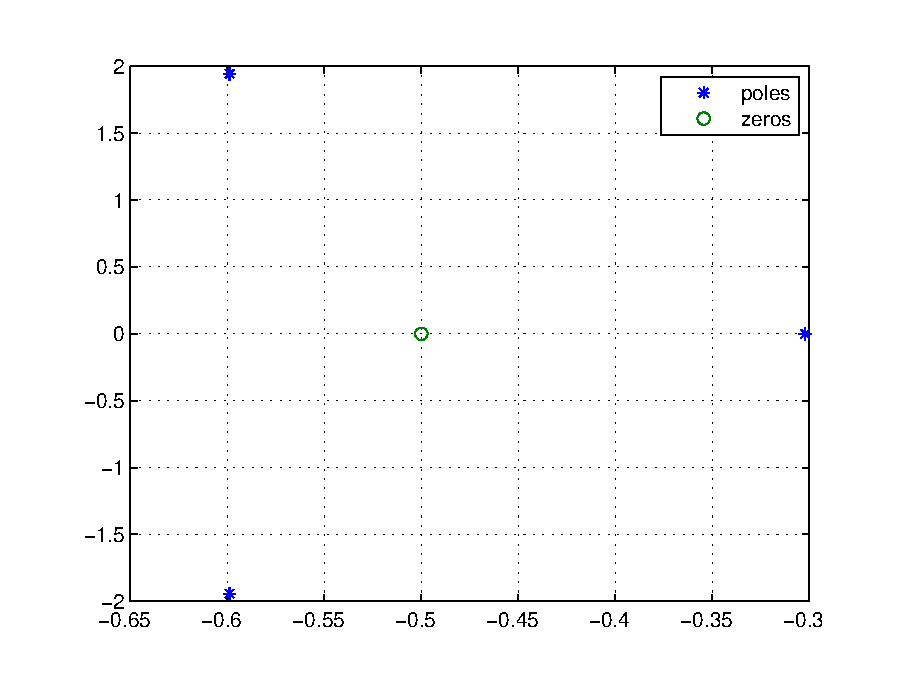
\includegraphics[scale=0.8]{image/pole2.eps}
        \caption{Нули и полюса}
    \end{figure}

    В таком случае набор корней будет следующим (также корни изображены на рисунке 5):
    \begin{align*}
        p_1 & = -0.5 & 
        z_1 & =  -0.3021 \\
        z_{2, 3} & =  -0.599 \pm j1.9441 &
    \end{align*} \par
    Как видно из рисунка 5 система устойчива. Степень устойчивости системы равна $Re(z_2) = Re(z_3) = -0.599$.

\parНа рисунке 6 и 7 представлены графики переходной и весовой функций замкнутой системы.

\begin{figure} [h!]
    \centering
    \begin{tikzpicture}
        \begin{axis} [
            width = \textwidth,
            height = 7cm,
            xlabel = {t, c},
            ylabel = {y},
            grid = major,
            grid style = {dashed},
            xmin = 0,  xmax = 30,
            extra y ticks = {0.39998, 0.419979, 0.379981},
            extra y tick labels = {0.4, 0.42, 0.38},
            extra x ticks = {7.2797},
            extra y tick style = {grid style = {black, dashed},font=\tiny},
            extra tick style={% changes for all extra ticks
                %tick align=outside,
                %tick pos=left,
                grid style={dotted,black}, 
            },
            ytick = {0, 0.1, 0.2, 0.3},
            xtick = {0, 2, 4, 6, 10, 12, 14, 16, 18, 20, 22, 24, 26, 28, 30},
        ]
            \addplot[blue, mark = none] table {data/step.txt};
            \draw[fill] (7.2797,0.38) circle(0.07cm);
        \end{axis}
    \end{tikzpicture}
    \caption{Переходная функция}
\end{figure}
\newpage
\begin{figure} [h!]
    \centering
    \begin{tikzpicture}
        \begin{axis} [
            width = \textwidth,
            height = 7cm,
            xlabel = {t, c},
            ylabel = {y},
            xmin = 0, xmax = 30,
            grid = major,
            grid style = {dashed},
            xmin = 0, 
            %xtick = {0, 5, 10, 15, 20, 25, 30, 35},
        ]
            \addplot[blue, mark = none] table {data/impulse.txt};
        \end{axis}
    \end{tikzpicture}
    \caption{Весовая функция} 
\end{figure}
Время переходного процесса $t_\text{п}=7.2797$. При выбранном коэффициенте $K=2.5$ перерегулирование отсутствует.
\par
Далее приведем модель (3) к модели ВСВ:
\begin{equation}
    \begin{cases}
        \dot{X} = \begin{bmatrix}
            -1.5 & 2 & 0\\
            1 & 0 & 0\\
            0 & 1 & 0\\
        \end{bmatrix}X + \begin{bmatrix}
            1\\
            0\\
            0\\
        \end{bmatrix}U \\
        y = \begin{bmatrix}0 & 1 & 0.5\end{bmatrix} X
    \end{cases}
\end{equation}
где $x = \begin{bmatrix} x_1 & x_2 & x_3 \end{bmatrix}^T$.
\par
Составим матрицы управляемости и наблюдаемости:

\begin{align*}
    W_y & = \begin{bmatrix}
        1 & -1.5 & 0.25\\
        0 & 1 & -1.5\\
        0 & 0 & 1\\
    \end{bmatrix} & 
    W_\text{н} & = \begin{bmatrix}
        0 & 1 & 0.5\\
        1 & 0.5 & 0\\
        -1 & -2 & 0\\
    \end{bmatrix}
\end{align*}
Ранги матриц равны $rang\{W_y\}=rang\{W_\text{н}\}=3$, значит, система полностью управляема и наблюдаема.

\newpage
\begin{center}
\section*{Выводы}
\end{center} \par
В лабораторной работе была исследована система 3-го порядка. С помощью соответствующих функций пакета Matlab были получены характеристики системы. 
\par 
Анализ разомкнутой системы показал, что система устойчива по корневому критерию. Исследовав АФЧХ, было выяснено, что система устойчива по критерию Найквиста.
\par 
При замыкании системы отрицательной обратной связью получили систему, устойчивость которой зависит от коэффициента $K$. С помощью критерия Гурвица определили допустимые значения $K$. В итоге был выбран $K=2.5$. При данном коэффициенте система имеет наилучшие параметры переходного процесса. Время переходного процесса минимально, а перерегулирование отсутствует. Корневые показатели подтверждают устойчивость системы.
\par 
Далее система была приведена с модели ВСВ. Анализ матриц управляемости и наблюдаемости показал, что система полностью управляема и наблюдаема.
\end{document}